\chapter{Verbal categories}
\label{chap:9}

\section{Tense"=aspect categories and their functions}
\label{sec:9-1}

Tense differentiation is in Palula, as in many other IA languages \citep[262]{masica1991}, secondary as compared to aspectual differentiation. Whereas aspect~-- or to be more precise, perfectivity~-- as an~inflectional element occurs next to the stem, followed by agreement suffixes, tense categories are, at least historically speaking, latecomers, and are still not fully part of the verb word in Palula. There is possibly one very visible and unexpected exception to this rule: the Present, which occurs with a~unique TMA"=marking morpheme that for various reasons should be viewed as a~marker of tense rather than aspect. Insofar as tense other than that is deemed relevant, it is indicated periphrastically by auxiliaries positioned after the finite verb (\sectref{subsec:9-1-5}).


\subsection{Basic tense"=aspect categories}
\label{subsec:9-1-1}


There are (as shown in \figref{fig:9-1}) three non"=periphrastic categories that can be considered basic: Future, Present and Perfective (Simple Past).

\begin{figure}[ht]
\centering
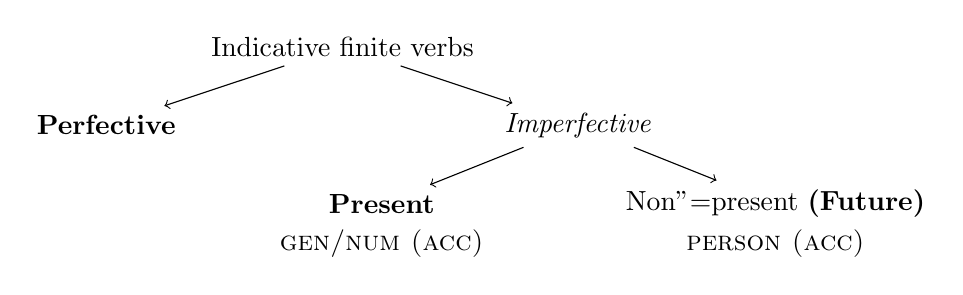
\begin{tikzpicture}
\node (d) at (1.5, 3) {\textbf{Perfective}};
\node (g) at (7.5, 3) {\textit{Imperfective}};
\node (h) at (5, 2) {\textbf{Present}};
\node (i) at (10, 2) {Non"=present \textbf{(Future)}};
\node (j) at (5, 1.5) {\textsc{gen/num (acc)}};
\node (k) at (10, 1.5) {\textsc{person (acc)}};
\node (n) at (4.5, 4) {Indicative finite verbs};
\foreach \from/\to in {g/h, g/i, n/d, n/g}
                   \draw [->] (\from) -- (\to);
\end{tikzpicture}
\caption{Basic non"=periphrastic tense"=aspect categories (bold type: inflectionally realised forms;
    \textsc{gen/num}: gender/number agreement; \textsc{erg}: ergative alignment; \textsc{acc}:
    accusative alignment)}
\label{fig:9-1}
\end{figure}

\subsection{Future}
\label{subsec:9-1-2}


Within the imperfective, the Future category in Palula is the morphologically unmarked counterpart of the Present, but it is also the periphrastically unmarked counterpart of the Past Imperfective (see \sectref{subsec:9-1-6}). 



This category is almost exclusively used in reference to future, i.e. not yet realised, situations, as in (\ref{ex:9-1}) and (\ref{ex:9-2}), whether close or distant in time, and covers intention as well as prediction \citep[105--108]{dahl1985}:

 \authcomm{In example \ref{ex:9-1}, I added a space between "[kh-úum]'' and "ta". Is this correct?}
\begin{exe}
\ex
\label{ex:9-1}
\gll ma nis áaǰ [kh-úum] ta rhootašíia ba kanaá [bh-úum]  \\
\textsc{1sg.nom} \textsc{3}\textsc{sg.prox.acc} today eat-\textsc{1sg} \textsc{prt} tomorrow  \textsc{prt} how become-\textsc{1sg} \\
\glt `If I eat it today, what will I then do tomorrow?' (A:HUB005)
\ex
\label{ex:9-2}
\gll theé míi baábu [máar-a] yaába tu [mhaar-íiṛ] yaába ṛó-(w)ee [máar-a] \\
then \textsc{1sg.gn} father die-3\textsc{sg} either 2\textsc{sg.nom} kill-2\textsc{sg }  or \textsc{3}\textsc{sg.dist.nom"=excl} die-\textsc{3}\textsc{sg}  \\
\glt `Then my father will die, either you will kill him or he himself will die.' (A:MAA013)
\end{exe}

While Present (\sectref{subsec:9-1-3}) is used for actions started but not yet seen as completed at the time of the utterance, the Future is used with reference to all future situations that have not yet commenced, such as the ones in (\ref{ex:9-3}), regardless of the degree of probability or volitionality. There is no other major construction in the language competing with this verb form.

\begin{exe}
\ex
\label{ex:9-3}
\gll ma aní šaak-á [háar"=um] ɡhooṣṭ-á har-í kúṛi anɡóor ǰheel-í tanaám the ɡúuli [th-íi] \\
\textsc{1sg.nom} \textsc{prox} wood-\textsc{pl} take-\textsc{1sg} house-\textsc{ob} take-\textsc{cv}  wife fire light-\textsc{cv } \textsc{3pl.rem.acc} to bread do-\textsc{3}\textsc{sg} \\
\glt `I will bring this wood to the house, and my wife is going to make a~fire and bake bread for
them.' (A:KIN017)
\end{exe}

Future is also often part of a~conditional expression as the apodosis verb (`will eat' in (\ref{ex:9-4})) and is sometimes used to express hopes and congratulations (as in (\ref{ex:9-5})), i.e. optative modality \citep[179]{bybeeetal1994}.

\begin{exe}
\ex
\label{ex:9-4}
\gll kasée ɡalé máaṭu dhraǰaá ba šúul-a the phedíl-u hée$\sim$ta hasó [khúu] \\
whose \textsc{prt} neck stretch.\textsc{cv} \textsc{prt} grass.heap-\textsc{ob}  to reach.\textsc{pfv"=msg } \textsc{condl} \textsc{3msg.rem.nom} eat.\textsc{3}\textsc{sg} \\
\glt `The one whose neck can reach to the heap of grass may eat.' (B:SHI016)

\ex
\label{ex:9-5}
\gll ṛe xu bíiḍ-i šúyi baát, mubaarák [bhíi] \\
\textsc{3fsg.rem.nom} \textsc{prt } much-\textsc{f} good.\textsc{f} talk blessing  become.\textsc{3}\textsc{sg} \\
\glt `That was very good [to hear], congratulations!' (A:CHN070717)
\end{exe}

\subsection{Present}
\label{subsec:9-1-3}

The only non"=periphrastic category that is primarily a~tense (and not an~aspect or mood) category is the Present, neither standing in a~direct morphological contrast with the Future nor the Perfective. Somewhat surprisingly, both from the perspective of languages at large \citep[103--128]{dahl1985} and IA comparative studies \citep[282, 288--289]{masica1991}, Present is the only category morphologically marked for tense (at least if analysed from a~synchronic perspective). It is as such one of the most frequently used verb forms and covers, within the temporal realm of the present, a~range of aspectual areas. 



Present typically refers to progressive situations, as illustrated in examples (\ref{ex:9-6})--(\ref{ex:9-7}),whether durative or punctual, with present time reference.

\begin{exe}
\ex
\label{ex:9-6}
\gll míi dáand-a [šila-yáan-a] \\
\textsc{1sg.gn} tooth-\textsc{pl} ache-\textsc{prs"=mpl} \\
\glt `I've got a~toothache.' (B:DHE5112)

\ex
\label{ex:9-7}
\gll tu ɡubáa [th-áan-u] \\
\textsc{2sg.nom} what do-\textsc{prs"=msg} \\
\glt `What are you doing?' (B:DHE1333)
\end{exe}

However, it also covers habitual situations, such as those in examples (\ref{ex:9-8}) and (\ref{ex:9-9}), which can be considered repeated on a~regular basis, at or after the time of the utterance: 

\begin{exe}
\ex
\label{ex:9-8}
\gll ma roošnaám raɣáṣṭi [uth-áan-u] uth-í ba ɣusulxaaná the [bayáan-u] \\
\textsc{1sg.nom} morning early get.up-\textsc{prs"=msg} get.up-\textsc{cv}  \textsc{prt} bathroom to go.\textsc{prs"=msg} \\
\glt `I get up early in the morning. After I get up I go to the bathroom.' (B:MOR001-2)

\ex
\label{ex:9-9}
\gll heewand-á dúu diṣṭ-í kir [dáan-u] \\
winter-\textsc{ob} two hand.span-\textsc{pl} snow give-\textsc{prs"=msg} \\
\glt `In the winter we [usually] get two hand"=spans of snow.' (B:HLN1015)
\end{exe}

The Present is also used for general statements (\ref{ex:9-10}) or sayings (\ref{ex:9-11}).

\begin{exe}
\ex
\label{ex:9-10}
\gll tarkaaṇ-íi dapáara bíiḍ-i saamaán [laɡaiǰ-éen-i]  \\
carpenter-\textsc{gn} sake much-\textsc{f} thing be.applied-\textsc{prs-f} \\
\glt `A carpenter needs a~lot of tools.' (A:HOW019)

\ex
\label{ex:9-11}
\gll har kaantíiru teeṇíi kráam šóo [ǰhaan-áan-u] \\
every fool \textsc{refl} work good.\textsc{msg} know-\textsc{prs"=msg} \\
\glt `Every fool knows his own work best.' (A:PRA004)
\end{exe}

Quite infrequently, Present is used in historical narratives, especially if describing a~situation from the perspective of a~role character. In (\ref{ex:9-12}) the narrator switches from the regular narration tense (i.e. the Perfective) to the Present:

\begin{exe}
\ex
\label{ex:9-12}
\gll eetáa wháat-u ta tsak"=tsák thaní áak šái wíi [tsak-áan-u] \\
there come.down-\textsc{pfv.msg} \textsc{prt} lick"=lick \textsc{qt} \textsc{idef}  thing water lick-\textsc{prs"=msg} \\
\glt `Coming down there he sees a~thing making sounds licking the water.' (A:PAS037)
\end{exe}

Present is used rather than the Future for imminent future reference, for instance, when someone is just about to do something, as when the speaker in (\ref{ex:9-13}) is just beginning to tell a~story.

\begin{exe}
\ex
\label{ex:9-13}
\gll típa ba ma tasíi paalaweeṇ-íi qiseé [th-áan-u] \\
now \textsc{prt} 1\textsc{sg.nom} 3\textsc{sg.gn} strong.man-\textsc{gn} story.\textsc{pl} do-\textsc{prs"=msg} \\
\glt `Now I'm going to tell you the story about this strong man.' (A:PAS029)
\end{exe}

\subsection{Perfective (Simple Past)}
\label{subsec:9-1-4}


The Perfective is primarily an~aspectually defined category, referring to events and actions completed before the time of the utterance. But it can alternatively be labelled a~Simple Past, as it is indeed restricted to past time reference \citep[79]{dahl1985}, and since it contrasts clearly with the Past Imperfective (see Section \sectref{subsec:9-1-6}) and other periphrastic categories that have relevance for more than one point in time, such as the Perfect and the Pluperfect (Sections \sectref{subsec:9-1-7}--\sectref{subsec:9-1-8}).



The Palula Perfective is used to refer to completed events in the past, whether remote or close in time. The examples (\ref{ex:9-14})--(\ref{ex:9-18}) illustrate the use of the Perfective, from the very remote event in (\ref{ex:9-14}), then gradually decreasing in remoteness in the following examples to the very close at hand reference in (\ref{ex:9-18}).

\begin{exe}
\ex
\label{ex:9-14}
\gll raaǰaá [múṛ-u] ta putr-óom tasíi hukumát [bulooṣṭéel-i] \\
king die.\textsc{pfv"=msg} \textsc{prt} son-\textsc{ob.pl} \textsc{3sg.gn} government snatch.\textsc{pfv-f} \\
\glt `When the king died the sons fought for the power [several hundred years ago].' (A:MAB003)

\ex
\label{ex:9-15}
\gll míi beenk-í qarzá [ɡhíin-u]  \\
\textsc{1sg.gn} bank-\textsc{ob} debt take.\textsc{pfv"=msg} \\
\glt `I took a~bank loan [several years ago].' (A:ISM003) 

\ex
\label{ex:9-16}
\gll xeer-á sanɡí [phedíl-u-eé] \\
happiness-\textsc{ob} with arrive.\textsc{pfv"=msg-q} \\
\glt `Did you arrive safely [some days ago]?' (A:CHN070104)

\ex
\label{ex:9-17}
\gll áaǰ índa ɡhuumaál [dít-i] xu xeér hín-u \\
today here earthquake give.\textsc{pfv-f} but safety be.\textsc{prs"=msg}  \\
\glt `Today there was an~earthquake here, but it's alright [earlier today].' (A:CHN070403)

\ex
\label{ex:9-18}
\gll ma tu sanɡí khoṇḍ-í bíiḍ-u xušaán [bhíl-u] \\
\textsc{1sg.nom} \textsc{2}\textsc{sg.nom} with speak-\textsc{cv} much-\textsc{msg} happy become.\textsc{pfv"=msg} \\
\glt `It was really nice to speak to you [the conversation that made the speaker happy is still going on at the time of the utterance.].' (A:CHN070104)
\end{exe}

It is also the category used for the main story line in narratives (whether historical or fictional), referring to sequences of events in the past, such as in (\ref{ex:9-19}).

\begin{exe}
\ex
\label{ex:9-19}
\gll deewúlii xálak"=am daawát [dít-i] atsharíit"=am the ki muqaabilá
th-íia  [thaníit-u] ta atshareet-íi paalawaaṇ-aán [ɡíia] paalawaaṇ-aán be deewúli [phedíl-a] \\
Dir.\textsc{gn} people-\textsc{ob.pl} invitation give.\textsc{pfv-f}  Ashreti-\textsc{ob.pl} to \textsc{comp} competition do-\textsc{1pl}  say.\textsc{pfv"=msg} \textsc{prt} Ashret-\textsc{gn} strong.man-\textsc{pl} go.\textsc{pfv.pl}  strong.man-\textsc{pl} go.\textsc{cv} Dir arrive.\textsc{pfv"=mpl} \\
\glt `The people of Dir issued an~invitation to have a~competition with them. The strong men of Ashret left and reached Dir.' (A:CHA001-3)
\end{exe}

Depending on the analysis, Perfective could also be said to include most types of conditionality. However, I have chosen to describe the conditional under non"=indicative categories (see \sectref{subsec:9-2-2}).


\subsection{Periphrastic tense"=aspect categories}
\label{subsec:9-1-5}

What I refer to as periphrastic tense"=aspect categories are those that are formed by a~finite inflected verb and one or more auxiliaries. While the so very central aspectual distinctions ``at the heart of the NIA verbal system'' \citep[262]{masica1991} very often are made morphologically and close to the verb stem, tense and mood are normally more peripherally marked functions in most modern IA languages. That is also the case with Palula, possibly with the exclusion of the morphologically marked Present (as was pointed out above). 



Interesting to note is that this may be a~relatively recent (or early stage of) grammaticalisation. We find the same principle applied in the two closely related varieties Sauji and Kalkoti, i.e. the addition of elements to the basic aspectual categories to obtain tense contrasts and to form Perfects and Pluperfects. Partly, however, we find other elements than those used in Palula, and in some cases, the former auxiliaries have become part of inflectional morphology and even fused with aspect suffixes. In Kalkoti, for instance, an \textit{s}-suffix (most certainly derived from the Past copula \textit{aas} `was, were') is added to the imperfective (mostly corresponding to Palula Present) to make it Past Imperfective, \textit{čuṇ-uun-s} `was writing', and to the Perfective (mostly corresponding to Palula Perfective) to make it Pluperfect, \textit{čuṇ-i-s} `had written' (the final consonant of the Perfective \textit{čuṇ-il} `wrote' has been dropped in phonological developments involving apocope and cluster reduction). There is generally speaking a~great variety among the Shina varieties in how the less central TMA categories have been grammaticalised. \citet[38]{schmidt2002} provides examples of forms of `be', `go' as well as `come' as origins of such grammaticalisations in the respective varieties. 



Tense, for instance, is mainly auxiliary, occurring outside the actual verb morphology (although this ``outside'' is not to be taken as an~absolute, as will be observed below when pointing out an~ongoing grammaticalisation process). The Present tense copula \textit{hin-} in its different agreement forms is used as a~present tense auxiliary (be.\textsc{prs}) and the (invariable) Past tense copula \textit{de} is used as a~Past tense auxiliary (\textsc{pst}).



Supplementing \figref{fig:9-1}, we now add the periphrastic marking (at least as far as tense is concerned) to get the fuller picture of the tense"=aspect dimensions relevant for the language, as illustrated in \figref{fig:9-2}. This characterisation is, however, a~slight simplification, as there are also resultative categories that are not taken into account as well as some dialectal differences between A. and B. that will be discussed in the following sections.


\begin{figure}[ht]
\centering
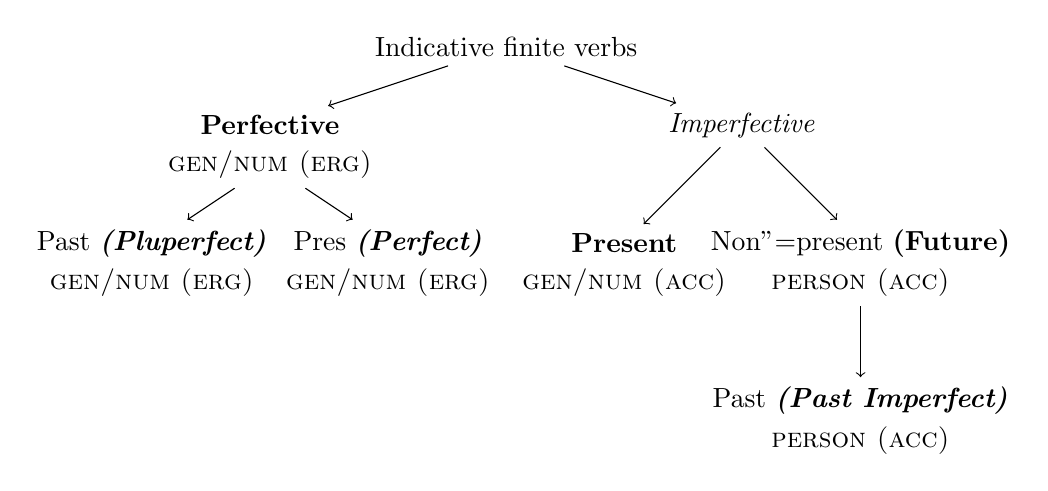
\begin{tikzpicture}
\node (a) at (0, 1) {\textsc{gen/num (erg)}};
\node (b) at (0, 1.5) {Past \textit{\textbf{(Pluperfect)}}};
\node (c) at (1.5, 2.5) {\textsc{gen/num (erg)}};
\node (d) at (1.5, 3) {\textbf{Perfective}};
\node (e) at (3, 1.5) {Pres \textit{\textbf{(Perfect)}}};
\node (f) at (3, 1) {\textsc{gen/num (erg)}};
\node (g) at (7.5, 3) {\textit{Imperfective}};
\node (h) at (6, 1.5) {\textbf{Present}};
\node (i) at (9, 1.5) {Non"=present \textbf{(Future)}};
\node (j) at (6, 1) {\textsc{gen/num (acc)}};
\node (k) at (9, 1) {\textsc{person (acc)}};
\node (l) at (9, -0.5) {Past \textit{\textbf{(Past Imperfect)}}};
\node (m) at (9, -1) {\textsc{person (acc)}};
\node (n) at (4.5, 4) {Indicative finite verbs};
\foreach \from/\to in {k/l, c/b, c/e, g/h, g/i, n/d, n/g}
                   \draw [->] (\from) -- (\to);
\end{tikzpicture}
\caption{Basic and periphrastic tense"=aspect categories (bold type: inflectionally realised forms;
  \textit{bold italics}: periphrastically realised forms; \textsc{gen/num}: gender/number agreement;
  \textsc{erg}: ergative alignment; \textsc{acc}: accusative alignment)\label{fig:9-2}}
\end{figure}

\subsection{Past Imperfective}
\label{subsec:9-1-6}

The Past Imperfective is formed by means of the person"=inflected imperfective verb stem (i.e. the Future verb form) followed by the invariable Past tense copula \textit{de}. It has two main functions, as a~past habitual (\ref{ex:9-20}) and a~past progressive (\ref{ex:9-21}).

\begin{exe}
\ex
\label{ex:9-20}
\gll míi so šúur máa-the bíiḍ-u šóo [ǰhóon-a de], ma ba tas the šóo [ǰhóon"=um de], máa-ee so mušqúl [bh-íia de] \\
\textsc{1sg.gn} \textsc{def.msg.nom} father.in.law \textsc{1sg.nom-}to much-\textsc{msg} good.\textsc{msg} know-\textsc{3sg} \textsc{pst} \textsc{1sg.nom} \textsc{prt} \textsc{3sg.acc}  to good.\textsc{msg} know-\textsc{1sg } \textsc{pst } \textsc{1sg.nom"=cnj}  \textsc{3sg.nom} on.terms become-\textsc{1pl} \textsc{pst} \\
\glt `That father"=in"=law of mine liked me a~lot, I liked him a~lot, and the two of us used to talk freely with each other.' (A:HUA006-8)

\ex
\label{ex:9-21}
\gll so kuṇaák bhešóol-u, bhešaá tasíi paaṇṭí [ɡaḍ-íi de], paaṇṭí ɡaḍ-í čhúuṇ-i tasíi ɡaḍ-í ba táa khóol-u so kuṇaák číɣi [d-íi de] \\
\textsc{def.msg.nom} child make.sit.\textsc{pfv"=msg} make.sit.\textsc{cv} \textsc{3sg.gn}  clothes take.off-\textsc{3sg } \textsc{pst} clothes take.off-\textsc{cv} put.\textsc{pfv-f}  \textsc{3sg.gn} take.off-\textsc{cv} \textsc{prt} there eat.\textsc{pfv"=msg}  \textsc{def.msg.nom} child crying give-\textsc{3sg} \textsc{pst} \\
\glt `He [an evil creature] made the child sit and there he was taking off its clothes. When he had taken them off and put them down he ate the child while it was crying.' (A:BRE005-6)
\end{exe}

An indication of an~ongoing grammaticalisation (or more correctly) morphologisation, by which the Past copula may become part of the verb morphology as a~past"=tense suffix \textit{(d-íi-de)}, is the fact that \textit{de} phonologically rather behaves like a~clitic than an~independent word, without independent word"=accent. In beginning attempts at writing the language, the inflected main verb has often been observed as written together with the copula auxiliary as if it were one word (while the more common tendency when writing Palula with an~Arabic"=based script is splitting rather than lumping), and it has become the topic of discussion among Palula writers whether this should be done or not. 


\subsection{Perfect}
\label{subsec:9-1-7}

The most common way of expressing the Perfect, i.e. a~reference to a~past (completed) event with current relevance, is by combining the Perfective verb form with the Present tense copula \textit{hin-} (at least that is the case in the A. dialect, while we shall have reason to return to the situation in the B. dialect). Both the Perfective verb and the auxiliary agree in gender and number with S (as in (\ref{ex:9-22})) or O (as in (\ref{ex:9-23}) and (\ref{ex:9-24})) according to an~ergative pattern.

\begin{exe}
\ex
\label{ex:9-22}
\gll míi baábu bi [wháat-u hín-u], salaám th-íi de \\
\textsc{1sg.gn} father also come.down.\textsc{pfv"=msg} be.\textsc{prs"=msg} greeting do-\textsc{3sg} \textsc{pst} \\
\glt `My father has also come, and he was telling you his greetings.' (A:CHN070309)

\ex
\label{ex:9-23}
\gll na ba asaám the ɡookhíi-am [dít-u hín-u] asaám the anú alaqá asím-ee teeṇíi zoor-í báandi ɡhiin-u-bháawu \\
\textsc{neg} \textsc{prt} \textsc{1pl.acc} to Chitrali-\textsc{ob.pl} give.\textsc{pfv"=msg}  be.\textsc{prs"=msg } \textsc{1pl.acc} to \textsc{prox.msg.nom} area  \textsc{1pl.erg"=excl} \textsc{refl} power-\textsc{ob} on take.\textsc{pptc"=msg"=adj} \\
\glt `Neither have the Chitralis given this to us, but it is an~area conquered with our very own power.' (A:ASH052)

\ex
\label{ex:9-24}
\gll islaám ba [aṭíl-i hín-i] ɡabarúuṭ-ii putr-óom \\
Islam \textsc{prt} bring.\textsc{pfv-f} be.\textsc{prs-f} Gabarut-\textsc{gn} son-\textsc{ob.pl} \\
\glt `It was Gabarut's sons who brought Islam.' (A:ASH054) 
\end{exe}

An extended use of the Perfect (like in a~number of other languages, \citealt[152]{dahl1985}) is inferential. In (\ref{ex:9-25}) it has actually stopped snowing, but it is inferred from looking at the ground on the morning after a~snowfall, that it must have been snowing during the night.

\begin{exe}
\ex
\label{ex:9-25}
\gll kir [dít-u hín-u] \\
snow give.\textsc{pfv"=msg} be.\textsc{prs"=msg} \\
\glt `It has been snowing.' (A:CHE070320)
\end{exe}

It is also used, instead of the Perfective (Simple Past), in some narratives, perhaps indicating the hearsay character~-- similar to the use of \textit{maní}~-- of the narrated content, as in (\ref{ex:9-26}), which is part of a~narrative where the Perfect is used throughout.

\begin{exe}
\ex
\label{ex:9-26}
\gll so utrap-í muṭ-á ǰe [ukháat-u hín-u] \\
\textsc{3sg.nom} run-\textsc{cv} tree-\textsc{ob} up go.up.\textsc{pfv"=msg} be.\textsc{prs"=msg} \\
\glt `He ran up into the tree.' (A:UNF008) 
\end{exe}

There is what appears to be a~parallel perfect form, used in a~very similar manner to the regular Perfect in (\ref{ex:9-27})--(\ref{ex:9-29}). This is formed by combining the Converb (\textsc{cv}) with the Present tense copula \textit{hin-}.

\begin{exe}
\ex
\label{ex:9-27}
\gll [mar-í hín-u], tas xudaái ubax-íi \\
die-\textsc{cv} be.\textsc{prs"=msg} \textsc{3sg.acc} God forgive-\textsc{3sg} \\
\glt `He has died, may God forgive him.' (A:ACR024)

\ex
\label{ex:9-28}
\gll zoór ǰanat-íi-e [yeyí hín-i] \\
power paradise-\textsc{ob"=gn} come.\textsc{cv} be.\textsc{prs-f} \\
\glt `Power has come from above.' (B:SHI019)

\ex
\label{ex:9-29}
\gll ɡíri ǰhulí xaamaár [dhreéɡ de hín-u] \\
rock on dragon stretched give.\textsc{cv} \textsc{prs"=msg} \\
\glt `The dragon was lying (outstretched) there on the rock.' (A:DRA009)
\end{exe}

It is possible that the focus is on the resulting stage rather than on the preceding event leading up to it in this construction, as it seems more commonly used with stative verbs and verbs with a~low degree of volitionality. It may therefore make more sense to see this as a~more lexically limited resultative construction \citep[135]{dahl1985} than a~pure perfect. In example (\ref{ex:9-29}) the temporal aspect is perhaps more that of a~pluperfect, `had stretched out'. 



Example (\ref{ex:9-30}) clearly illustrates the use of this resultative constructing. Here the resulting absence of the husbands is focused, rather than their going away. The translation `our husbands are gone' seems more natural than `our husbands have gone'. Note also how it interacts with the Past Imperfective as the tense"=aspect category used for the waiting of the women and children at home, and the Future is used for the hoped for outcome in the form of fresh meat being brought home.

\begin{exe}
\ex
\label{ex:9-30}
\gll díiš-a ba baalbač-á kuṛíina tamá th-éen de: asée bharíiw-a [be hín-a] neečíir the whaal-éen mhaas-á whaal-éen \\
village-\textsc{ob} \textsc{prt} child-\textsc{pl} women.\textsc{pl} waiting  do-\textsc{3pl} \textsc{pst } \textsc{1pl.gn} husband-\textsc{pl} go.\textsc{cv} \textsc{prs"=mpl}  hunt do.\textsc{cv} bring.down-\textsc{3pl} meat-\textsc{pl} bring.down-\textsc{3pl} \\
\glt `In the village the women and children were waiting, (saying) ``Our husbands are gone for a~hunt. They will bring home meat''.' (B:AVA218)
\end{exe}

When used with a~motion verb such as `get up', the Converbal construction brings forth the ``adjectival'' meaning `is standing', as in (\ref{ex:9-31}).

\begin{exe}
\ex
\label{ex:9-31}
\gll ak čhéeli maidúun-a wée du"=khur-áam ǰhulí [uth-í hín-i] \\
\textsc{idef} goat field-\textsc{ob} in two"=foot-\textsc{ob.pl} on get.up-\textsc{cv} be.\textsc{prs-f} \\
\glt `A goat has got up [i.e. is standing] on two feet in the field.' (B:SHB721)
\end{exe}

The interesting thing, however, is that the ``regular'' Perfect as described in the beginning of this section, seems to be missing altogether in the B. dialect. Instead, the Converbal construction is widely used with intransitive verbs, as in the examples (\ref{ex:9-27})--(\ref{ex:9-28}) and (\ref{ex:9-30})--(\ref{ex:9-31}), and probably marginally also with transitive verbs, as in (\ref{ex:9-32})--(\ref{ex:9-33}) (although my B. data is too limited to the genre of narrative discourse to provide a~clear indication).

\begin{exe}
\ex
\label{ex:9-32}
\gll ma ɡúuli [khaá hín-u] (=khaánu)  \\
\textsc{1sg.nom} bread eat.\textsc{cv} be.\textsc{prs"=msg} \\
\glt `(Yes,) I have eaten.' [= `I have been eating already', as an~answer to a~question or an~invitation to eat.] (B:DHE2170)

\ex
\label{ex:9-33}
\gll ma na [niweš-í hin-u] thaníit-u  \\
\textsc{1sg.nom} \textsc{neg} write-\textsc{cv} be.\textsc{prs"=msg} say.\textsc{pfv"=msg} \\
\glt `I have not written [referring to some suspicious letters], he said.' (B:LET027)
\end{exe}

Note that this construction, again focusing on the result rather than on the event itself, is based on a~transitive imperfective stem and therefore requires an~accusative agreement pattern, while the agreement with the regular Perfect, using the perfective transitive stem is ergative. But there is also another (possibly more ``regular'' or lexically less restricted) Perfect used in this dialect formed with Converb+\textit{heensíl-} (the Perfective of the intransitive verb \textit{háans}- `stay, live, exist') as in (\ref{ex:9-34}).

\begin{exe}
\ex
\label{ex:9-34}
\gll ma [khaá heensíl-u]  \\
\textsc{1sg.nom} eat.\textsc{cv} stay.\textsc{pfv"=msg} \\
\glt `I have eaten.' (B:HLE1034)
\end{exe}

Even the A. variety has this construction (but with an~added Present copula), used in some instances of hearsay as in (\ref{ex:9-35}) or inferentially (by seeing water on the ground and subsequently reporting it to another person who has not been able to infer it), as in (\ref{ex:9-36}), but possibly still in free variation with the ``regular'' Perfect:

\begin{exe}
\ex
\label{ex:9-35}
\gll so tas khúṭ-a wée [čuk-í heensíl-u hín-u] \\
\textsc{3msg.nom} \textsc{3sg.acc} leg-\textsc{ob} in bite-\textsc{cv} stay.\textsc{pfv"=msg} be.\textsc{prs"=msg} \\
\glt `It (so he said) bit him in the leg.' (A:TAQ178)

\ex
\label{ex:9-36}
\gll áaǰ peexáur-a [muč-í heensíl-u hín-u]  \\
today Peshawar-\textsc{ob} rain-\textsc{cv} stay.\textsc{pfv"=msg} be.\textsc{prs"=msg} \\
\glt `Today it has been raining in Peshawar.' (A:CHE070320)
\end{exe}

\subsection{Pluperfect}
\label{subsec:9-1-8}

While the regular Perfect is the perfective with relevance for the present situation, the Pluperfect is the perfective with relevance for a~past situation. This is also reflected in the formal expression: Perfect is formed with the perfective verb and a~Present tense copula, and the Pluperfect is formed with the Perfective verb and a~Past tense copula \textit{de} `was, were'. 


The contrast between these is illustrated in (\ref{ex:9-37}) and (\ref{ex:9-38}). (\ref{ex:9-37}) refers to an~event with present time relevance and a~still visible result, a~recently painted house, hence Perfect, while (\ref{ex:9-38}) has past time relevance only, i.e. a~house that was built but had been torn down prior to the utterance, hence Pluperfect.

\begin{exe}
\ex
\label{ex:9-37}
\gll aní ɡhooṣṭ-á ráanɡ kií [dít-u hín-u]  \\
\textsc{prox} house-\textsc{ob} paint who.\textsc{ob} give.\textsc{pfv"=msg} be.\textsc{prs"=msg} \\
\glt `Who painted this house?' (A:TAQ130)

\ex
\label{ex:9-38}
\gll anú ɡhoóṣṭ kií [samóol-u de] \\
\textsc{prox.msg.nom} house who.\textsc{ob} build.\textsc{pfv"=msg} \textsc{pst} \\
\glt `Who built this house?' (A:TAQ129)
\end{exe}

In narratives, the Pluperfect is used to refer to an~event taking place prior to, and thus contrasting with, the time line of the story (which normally would be related with the Perfective), as in (\ref{ex:9-39}).

\begin{exe}
\ex
\label{ex:9-39}
\gll atáa ɡíia ta dóodu ayaan"=miír ta ǰáand-u hín-u, xaamaár ba [mheeríl-u de] \\
there go.\textsc{pfv.pl} \textsc{prt} grandfather Ayan.Mir \textsc{prt}  alive-\textsc{msg}
be.\textsc{prs"=msg} dragon \textsc{prt} kill.\textsc{pfv"=msg} \textsc{pst} \\
\glt `When they came there, grandfather Ayan Mir was alive, but the dragon had been killed.' (A:AYB044) 
\end{exe}

There seems to be a~drift towards a~use of Pluperfect as a~general remote past, not an~uncommon development generally \citep[147]{dahl1985}, and in the region in particular. However, that is not to say that the two constructions~-- Perfective (Simple Past) and Pluperfect~-- would therefore be in totally free variation when referring to remote past, although I am not able to pinpoint exactly where the dividing line goes. The utterance (\ref{ex:9-40}) is an~answer to the question whether the speaker had met the other person recently, and it could perhaps be that it is the temporal adverbial phrase that somehow favours the Pluperfect, but this is so far only speculative on my part.

\begin{exe}
\ex
\label{ex:9-40}
\gll áak haftá muṣṭú [dhríṣṭ-u de]  \\
one week back see.\textsc{pfv"=msg} \textsc{pst} \\
\glt `(I) saw him a~week ago.' (A:CHN070110)
\end{exe}

Another possible indication of which category to use seems to be related to whether or not a~measurable chunk of time (exactly how long is probably not that important) can be considered to have elapsed between the event~-- or the end"=point of the event if durative~-- and the time of reference, as contrasted with the event coinciding too closely with the time of reference. This again points to the Pluperfect as developing a~secondary sense of temporal remoteness. This can be seen when comparing (\ref{ex:9-41}) and (\ref{ex:9-42}) (both part of the questionnaire prepared by \citet{dahl1985} and applied to Palula), where the former uses the Perfective and the latter the Pluperfect.

\begin{exe}
\ex
\label{ex:9-41}
\gll \label{bkm:Ref190742986}dhoóṛ ma yhóol-a díi muṣṭú tíi dúu xat-í [čooṇṭéel"=im] \\
yesterday 1\textsc{sg.nom} come.\textsc{pptc"=ob} from back \textsc{3sg.ob} two letter-\textsc{pl} write.\textsc{pfv"=fpl} \\
\glt `When I came yesterday, he had (just) written two letters.' (A:TAQ138)

\ex
\label{ex:9-42}
\gll dhoóṛ ma ɡhooṣṭ-a yhóol-u ta tíi dúu xat-í [čooṇṭéel"=im de] \\
yesterday 1\textsc{sg.nom} house-\textsc{ob} come.\textsc{pfv"=msg}  \textsc{prt} \textsc{3sg.ob} two letter-\textsc{pl} write.\textsc{pfv"=fpl} \textsc{pst} \\
\glt `When I came home yesterday, he had written two letters (during my absence).' (A:TAQ139)
\end{exe}

However, it is also possible to describe the difference as being one of perspective. In (\ref{ex:9-41}) the utterance can be said to describe what took place during the time before my arrival, whereas (\ref{ex:9-42}) describes the resulting situation at my arrival.


Again, although this particular form of the Pluperfect does occur in the B. dialect, it seems markedly less frequent than in the A. dialect. There is also another construction in B., illustrated in (\ref{ex:9-43}) and (\ref{ex:9-44}), somewhat parallel to the Converb+\textit{heensíl}-construction above, but with an~additional Past tense copula, which certainly shares at least some of the semantic characteristics of the ``regular'' Pluperfect in A. (the phonologically reduced alternative form \textit{khasúlde} in (\ref{ex:9-44}) may point to an~ongoing grammaticalisation).

\begin{exe}
\ex
\label{ex:9-43}
\gll bíiḍ-u purúuṇ-u maasṭér, so baraaníi-e waxt-íi-e sabáq [man-í heensíl-u de] \\
much-\textsc{msg} old-\textsc{msg} teacher 3\textsc{msg.nom}  foreigner-\textsc{gn}
time-\textsc{ob"=gn} lesson say-\textsc{cv} stay.\textsc{pfv"=msg} \textsc{pst} \\
\glt `He was a~very old teacher, he had studied during the British rule.' (B:LET003)

\ex
\label{ex:9-44}
\gll ma ɡúuli [khaá heensíl-u de](=khasúlde) \\
\textsc{1sg.nom} bread eat.\textsc{cv} stay.\textsc{pfv"=msg} \textsc{pst}  \\
\glt `I had eaten (already).' (B:DH5378)
\end{exe}

\section{Non"=indicative finite categories and their functions}
\label{sec:9-2}


Not all of the following categories are equally central or to the same extent grammaticalised, but they are all somehow part of the modal realm within the TMA system and thus deserve to be mentioned together in one place.


\subsection{Imperative}
\label{subsec:9-2-1}

The bare Imperative, in its two forms \textsc{sg} ((\ref{ex:9-46}) and (\ref{ex:9-47})) and \textsc{pl (}(\ref{ex:9-45}) and (\ref{ex:9-48})\textsc{)}, is mainly used for commands (\ref{ex:9-45}) and not overly polite requests (\ref{ex:9-46})--(\ref{ex:9-48}).

\begin{exe}
\ex
\label{ex:9-45}
\gll koó hin-eé [yh-óoi]  \\
who.\textsc{nom} be.\textsc{prs"=mpl.q} come-\textsc{imp.pl}  \\
\glt `If there is anyone (who is ready to take up the challenge), come!' (A:JAN038)

\ex
\label{ex:9-46}
\gll amzarái seéb zeerí th-áan-u ki eé insaán ma [uṛí] \\
lion sir supplication do-\textsc{prs"=msg} \textsc{comp} oh  man \textsc{1sg.nom} let.out.\textsc{imp.sg} \\
\glt `Sir Lions is begging: Oh man, set me free!' (A:KIN025)

\ex
\label{ex:9-47}
\gll anís míi doost-á the [phedá] \\
\textsc{3sg.prox.acc} \textsc{1sg.gn} friend-\textsc{ob} to make.reach.\textsc{imp.sg} \\
\glt `Take this (one) to my friend!' (B:FLW797)

\ex
\label{ex:9-48}
\gll man-éen-i ki ma patú [yh-óoi], ma [saat-óoi] \\
say-\textsc{prs-f} \textsc{comp} \textsc{1sg.nom} after come-\textsc{imp.pl} \textsc{1sg.nom} take.care-\textsc{imp.pl} \\
\glt `It (the goat) says: Come after me, take care of me!' (A:KEE007-8)
\end{exe}

Normally, it seems, the second person is not explicitly expressed with a~pronoun in imperative clauses, but occasionally it does occur, as in (\ref{ex:9-49}).

\begin{exe}
\ex
\label{ex:9-49}
\gll míi maníit-u ki šóo [tus b-óoi] \\
\textsc{1sg.gn} say.\textsc{pfv"=msg} \textsc{comp} good.\textsc{msg} \textsc{2pl.nom} go-\textsc{imp.pl} \\
\glt `I said: You may go!' (A:ACR010)
\end{exe}

The \textsc{pl} form is always used with reference to more than one person, but a~more polite request could be done by adding the suffix/particle \textit{neé} or \textit{na}, to any of the two forms, to the singular in (\ref{ex:9-50}) and to the plural in (\ref{ex:9-51}).

\begin{exe}
\ex
\label{ex:9-50}
\gll tu [dac̣h-á neé] \\
\textsc{2sg.nom} look-\textsc{imp.sg} \textsc{hon}  \\
\glt `You take a~look!' (A:AYB012)

\ex
\label{ex:9-51}
\gll dar [muč-úui neé] \\
door open-\textsc{imp.pl} \textsc{hon} \\
\glt `Open the door, please!' [uttered by a~little girl addressing older women, supposedly mother and grandmother, in the household] (B:HLN1020)
\end{exe}

The Imperative is regularly negated with the negation particle \textit{na}, as in (\ref{ex:9-52}), and there is therefore no prohibitive category distinct from the Imperative in the language.

\begin{exe}
\ex\authcomm[noline]{Please check the characters in this word. Is {\glqq}širinɡ\'{á}{\grqq} correct?}
\label{ex:9-52}
\gll kúṛi the maníit-u ki teeṇíi banɡleé [na širinɡ\'{á}] \\
woman to say-\textsc{pfv"=msg} that \textsc{refl} bracelet.\textsc{pl} \textsc{neg} rattle.\textsc{imp.sg} \\
\glt `He said to the woman: Don't rattle your bracelets!' (A:WOM643)
\end{exe}

\subsection{Conditional}
\label{subsec:9-2-2}

Conditionality is essentially expressed with the protasis verb in a~conditional clause in the Perfective (or one of the periphrastic categories built on it), while the apodosis verb may be in the Present or the Future, a ``split tense/aspect reference'' not uncommon in languages overall (e.g. in Arabic, \citealt[80]{dahl1985}). It is commonly, in such constructions, used together with an~additional element that can be analysed alternatively as a~subjunction, alternatively as an~auxiliary. There are two such elements in Palula, one \textit{sée$\sim$ta} (B. \textit{síinta}) which is used to form constructions of assumed conditionality, \textit{yhóolu sée$\sim$ta} `if he comes, when coming' (\ref{ex:9-53}) and another, \textit{hée$\sim$ta}, which usually carries a~hypothetical meaning, \textit{dítu hée$\sim$ta} `if you would give, were you to give' (\ref{ex:9-54}). Further details on conditionality can be found in \sectref{subsec:13-4-4}. 

\begin{exe}
\ex
\label{ex:9-53}
\gll misrí [yhóol-u sée$\sim$ta] misrí díi tsaṭák hóons-a \\
mason come.\textsc{pfv"=msg} \textsc{condh} mason from hammer stay-\textsc{3sg} \\
\glt `When the mason comes he would have a~hammer (i.e. he would bring a~hammer with him).' (A:HOW010)

\ex
\label{ex:9-54}
\gll bíiḍ-u táru bi [dít-u hée$\sim$ta] xaraáb bh-éen-i \\
much-\textsc{msg} fast also give.\textsc{pfv"=msg} \textsc{condl} bad become-\textsc{prs-f} \\
\glt `If it (salt) is given very soon it will harm her (the goat).' (A:KEE019)
\end{exe}

\subsection{Obligative}
\label{subsec:9-2-3}

Whether or not the verb form coding the Obligative should be seen as a~finite or a~nonfinite verb form is not as straightforward a~matter as it may first seem. It is analysable as both, and it is possible that we are witnessing a~still ongoing development from one to the other. 



The function of the Obligative is to express obligation, need or predestination to carry out a~particular action. This is the agent"=oriented modality expressed in languages at large, though not necessarily inflectionally \citep[177--187]{bybeeetal1994}. Often in IA languages this particular semantics is connected with what \citet[322]{masica1991} refers to as a \textit{future passive participle (of obligation)}, which behaves like an~adjective, but may in some languages be formally identical with a~Verbal Noun, as is the case with the Urdu"=Hindi infinitive formed with \textit{-nā}. 



In Palula, the Obligative is used both in the personal sense `scheduled to, is to' (\ref{ex:9-55}) and in a~more general or impersonal sense of `ought to, one should' (\ref{ex:9-56}).

\begin{exe}
\ex
\label{ex:9-55}
\gll muníir"=ii rhootašíia dhruú$\sim$ṣ-a the [b-eeṇḍeéu] \\
Munir-\textsc{gn } tomorrow Drosh-\textsc{ob} to go-\textsc{oblg} \\
\glt `Munir has/is to go to Drosh tomorrow.' (A:HLE3059)

\ex
\label{ex:9-56}
\gll kháač-a kráam-a díi ba teeṇíi zaán bač [th"=eeṇḍeéu] \\
bad-\textsc{ob} work-\textsc{ob} from \textsc{prt} \textsc{refl} self safe do-\textsc{oblg} \\
\glt `One should avoid ( =save oneself from) evil actions.' (A:SMO023)
\end{exe}

Sometimes the future reading of `will inevitably happen' is clearly present, as in (\ref{ex:9-57}), while in other cases there is no such future sense, only an~instructional one with the sense of `the way it should be/usually is being done', as in (\ref{ex:9-58}).

\begin{exe}
\ex
\label{ex:9-57}
\gll so mhaás aaxér xátum [bh"=eeṇḍeéu] bhíl-u \\
\textsc{def.msg.nom} meat end finished become-\textsc{oblg} become.\textsc{pfv"=msg}  \\
\glt `The meat was doomed to finish in the end.' (A:THA008)

\ex
\label{ex:9-58}
\gll páanǰ sáat ba bheénš [laɡay"=aiṇḍeéu] \\
five seven \textsc{prt} beam apply-\textsc{oblg} \\
\glt `Then a~five by seven beam is attached.' (A:HOW076)
\end{exe}

The dual syntactic character of the construction is seen if we compare (\ref{ex:9-55}) with (\ref{ex:9-57}). In (\ref{ex:9-55}) it is noun"=like (`Munir's inevitable going to Drosh'), with the agent in the genitive, whereas in (\ref{ex:9-57}) it is adjective"=like (`the inevitably finishing meat'). It is also in the first instance where the Obligative is most finite, whereas its finiteness can be questioned in the second one.


It seems the agent is generally avoided with Obligative transitive verbs, and as such is also becoming an~alternative way of expressing a~passive meaning (cf. \sectref{subsec:8-5-2}), with sense of ability (or inability) rather than of obligation. I would still hold that Obligative is primarily modality and only secondarily voice. Possibly related to the degree of obligation is an~alternation between the coding of the agent in the nominative (\ref{ex:9-59}) versus the genitive coding we saw above (\ref{ex:9-55}).

\begin{exe}
\ex
\label{ex:9-59}
\gll so típa [b-eeṇḍeéu] \\
\textsc{3sg.nom} now go-\textsc{oblg} \\
\glt `He's about to leave./He must leave now.' (A:Q9.0003)
\end{exe}

In my data I do not have any clear examples of transitive verbs showing the same alternations, but as far as the agent is at all explicitly mentioned, he/she always occurs in the genitive. However, \citet[24]{morgenstierne1941} gives examples of a~few transitive Obligatives where it seems the nominative and the genitive are equally possible, while his subjects of intransitive Obligatives invariable occur in the nominative\footnote{Although we can exclude the genitive, we in fact do not know, due to the absence of such examples, whether any pronouns other than the \textsc{1sg} (which lacks a~nom/acc contrast) would have been coded in the nominative or accusative in those days (the 1920s).}: \textit{mī / ma krām thäiṇḍēu} `I must(?) do the work'; \textit{mī / ma wī piläiṇḍēu (hinu)} `I can(?) drink water'; \textit{āǰ ma y[25B?]ṇḍēu hinu} `I can (or must) come to"=day'.


\subsection{Hearsay and ``quotative''}
\label{subsec:9-2-4}

Hearsay, formed with \textit{maní} is grammaticalised to a~much lower extent than the hitherto mentioned categories, and is thus only in a~peripheral sense part of the TMA system. When it occurs, it occurs at the end of a~sentence, like an~auxiliary, thus after the inflected finite verb form (whether simple or periphrastically formed) to indicate reported (but not self"=experienced) information. It is chiefly (but optionally) used in narratives, especially those of a~legendary character, and mostly at the beginning of such a~narrative, which is seen in (\ref{ex:9-60}).\footnote{I am inclined not to consider it a~story starter as such; that function is instead carried by \textit{bíiḍu muṣṭú, muṣṭú zamaanéyii}, \textit{muxáak zamaanée} or similar more or less standardised story"=starters. Also the initial sentence(s) occurrence of the participant"=introduction \textit{heensílu de} `there was' is typical of the Palula storytelling discourse.} 

\begin{exe}
\ex
\label{ex:9-60}
\gll \label{bkm:Ref190746425}bíiḍ-u muṣṭú áak miiš-íi áak dhií de [maní] \\
much-\textsc{msg} before \textsc{idef} man-\textsc{gn} \textsc{idef} daughter be.\textsc{pst}
\textsc{hsay} \\
\glt `A long time ago there was a~man who had a~daughter.' 

\gll se áak bakaraál phoó the ašáq de [maní] \\
\textsc{3fsg.nom} \textsc{idef} shepherd boy to love be.\textsc{pst} \textsc{hsay} \\
\glt `She was in love with a~shepherd boy.'

\gll so phoó bi tás the bíiḍ-u  šóo ǰhóon-a de \\
\textsc{def.msg.nom} boy also \textsc{3sg.acc} to much-\textsc{msg}  good.\textsc{msg} know-\textsc{3sg} \textsc{pst} \\
\glt `The boy too liked her very much.' (A:SHY001-3)
\end{exe}

As can be seen in example (\ref{ex:9-60}), \textit{maní} is used only in the two first sentences, but there are also narratives where this is used much more frequently, in the extreme case after almost all sentences. It is also used when presenting legendary or questionable facts in a~narrative, as in (\ref{ex:9-61}), otherwise unmarked in this respect.

\begin{exe}
\ex
\label{ex:9-61}
\gll tasíi áaṣṭ zára kuṇaak-á heensíl-a de [maní] \\
3\textsc{sg.gn} eight thousand.\textsc{pl} child-\textsc{pl} stay.\textsc{pfv"=mpl} \textsc{pst} hsay \\
\glt `He had 8,000 children (it has been said).' (A:ABO008)
\end{exe}

It is, however, not restricted to narrative discourse. It may be used in any everyday conversation, as in (\ref{ex:9-62}) with the Perfect. Also in this utterance it is only after the first finite verb form that the hearsay marker/auxiliary occurs.

\begin{exe}
\ex
\label{ex:9-62}
\gll asíi atshareet-á bíiḍ-u kir [dít-u hín-u maní], hiimeel-í bi whéet"=im hín-i \\
\textsc{1pl.gn} Ashret-\textsc{ob} much-\textsc{pl} snow give.\textsc{pfv"=msg} be.\textsc{prs"=msg} \textsc{hsay} glacier-\textsc{pl} also come.down.\textsc{pfv"=fpl} be.\textsc{prs-f} \\
\glt `(I have been told that) a~lot of snow has fallen in our (village) Ashret, and there have been
avalanches as well.' (A:CHN070320)
\end{exe}

Related to this issue, is the use of the quotation marker \textit{thaní}, with a~very similar etymology, which may develop into an~auxiliary. Triggered by the verb"=final word order, it may become restricted to the position after the finite verb and become narrowed down to this particular verb form (now it is alternatively expressed with other verb forms). In the process it may also become a~marker of a~more grammaticalised inferentiality category, as such contrasting with hearsay, rather than now as chiefly a~marker of direct quotation/perception (see \sectref{subsec:13-5-1}). In (\ref{ex:9-63}) it has taken on a~function beyond mere quotation.

\begin{exe}
\ex
\label{ex:9-63}
\gll so búd-u ki míi kúṛi dúi koó [ɡaḍ-í ɡhin-í ɡíia thaní]  \\
\textsc{3msg.nom} understand.\textsc{pfv"=msg} \textsc{comp} \textsc{1sg.gn} woman  other someone pull-\textsc{cv} take-\textsc{cv} go.\textsc{pfv.pl} \textsc{qt} \\
\glt `He understood, that someone else had taken his wife away.' (A:WOM656)
\end{exe}

The grammaticalisation of Hearsay as well as other types of inferentiality is documented for a~number of other languages in the region, especially in the geographically adjacent Khowar and Kalasha, where it is particularly well"=developed and is an~integral part of verb morphology \citep{bashir1996}. 


\section{Nonfinite forms and their functions}
\label{sec:9-3}

Most of the nonfinite verb forms have implications for syntax and are hard to define functionally without discussing syntactic structure. The following sections therefore only aim at giving a~basic characterisation of their function; where to find them in the grammatical system and what their further inflectional properties are, wherever the latter is relevant. For further details in this regard, the cross"=references given at the end of each subsection should be consulted. 


\subsection{Converb (Conjunctive Participle) }
\label{subsec:9-3-1}


The Converb (defined by \citet{haspelmath1995} as ``a nonfinite verb form whose main function is to mark adverbial subordination'') is essentially a~perfective adverbial participle (cf. the Copredicative Participle, \sectref{subsec:9-3-5}, which is an~imperfective adverbial participle). It carries an~approximate meaning of `having done, etc.' and is, as in many other IA languages \citep[323, 397--401]{masica1991}, where it often is referred to as a~Conjunctive Participle,\footnote{The identification of the corresponding verb form in Kohistani Shina (otherwise referred to as a~Conjunctive Participle) with the Converb, according to \citeauthor{haspelmath1995}'s (\citeyear{haspelmath1995}) definition, is carried through in \citet{schmidt2003}.} a~characteristic, very frequently occurring and syntactically important nonfinite verb form. It is (as \citeauthor{haspelmath1995}'s definition also spells out) especially important in adverbial subordination and in expressing perfective sequentiality, as illustrated in (\ref{ex:9-64}) (see \sectref{subsec:13-3-1} and \sectref{subsec:13-4-1} for further details).

\begin{exe}
\ex
\label{ex:9-64}
\gll aḍaphará [whayí] ba damá thíil-u \\
halfways come.down.\textsc{cv} \textsc{prt} pause do.\textsc{pfv"=msg} \\
\glt `We rested when we had come down halfways.' (A:GHA057)
\end{exe}

It is also a~component in some resultative constructions mentioned above (\sectref{subsec:9-1-7}) as well as in compound verbs (\sectref{subsec:8-6-2}), and is possibly a~source for the grammaticalisation of verbs to postpositions.


\subsection{Perfective Participle}
\label{subsec:9-3-2}


Since the Perfective Participle is formally identical to the Perfective (and as such has become a~finite verb form), it only occurs marginally in what must be interpreted as a~nonfinite function. When it does, such as in the (Perfective) nominalisation below, it can also (but only optionally) be inflected for case, genitive in (\ref{ex:9-65}) and oblique in (\ref{ex:9-66}).

\begin{exe}
\ex
\label{ex:9-65}
\gll eetás [samóol-íi] pahúrta \\
\textsc{3sg.rem.acc} build-\textsc{pptc"=gn} after \\
\glt `After the (completed) construction of it{\ldots}' (A:HOW044)

\ex
\label{ex:9-66}
\gll dhoóṛ ma [yhóol-a] díi muṣṭú tíi dúu xat-í čooṇṭéel"=im \\
yesterday 1\textsc{sg.nom} come.\textsc{pptc"=ob} from back \textsc{3sg.ob} two letter-\textsc{pl} write.\textsc{pfv"=fpl} \\
\glt `When I came yesterday, he had (just) written two letters.' (A:TAQ138)
\end{exe}

The Perfective Participle is also, as seen in (\ref{ex:9-67}), used attributively in some relativisations (see \sectref{subsec:13-6-6} for further details).

\begin{exe}
\ex
\label{ex:9-67}
\gll phaí teeṇíi háat"=am [čooṇṭéel-i rumiaál] dít-i hín-i \\
girl \textsc{refl} hand-\textsc{ins} embroider.\textsc{pptc-f} handkerchief give.\textsc{pfv-f} be.\textsc{prs-f} \\
\glt `The girl gave [him] the handkerchief which she herself had embroidered.' (A:SHY031)
\end{exe}

Often however, as can be seen in (\ref{ex:9-68}), the Perfective Participle will occur with an~additional adjectiviser \textit{bháau} or \textit{wáandu/wéendi}, maybe to mark it off as different from the otherwise formally identical Perfective.

\begin{exe}
\ex
\label{ex:9-68}
\gll muṣṭú zamanáyii paṇardóoṛ-a búuḍ-a ɡáaḍ-a xalk-íim díi qisá [ṣuunt-u-wáand-u] áa eeteeṇ-ú hín-u ki \\
back period.\textsc{gn} elder-\textsc{pl} old-\textsc{pl} big-\textsc{pl}  people-\textsc{pl.ob} from story hear.\textsc{pptc"=msg"=adj"=msg} \textsc{idef} such-\textsc{msg} be.\textsc{prs"=msg} \textsc{comp} \\
\glt `Once, a~story goes, which has been heard from the elders, the old and the powerful people{\ldots}.'
(A:KIN001)
\end{exe}

Some Perfective Participles have been fully lexicalised as adjectives: \textit{šúku} `became dry' {\textgreater} `dry', \textit{páaku} `ripened' {\textgreater} `ripe', \textit{khíndu} `became tired' {\textgreater} `tired', etc.


\subsection{Verbal Noun}
\label{subsec:9-3-3}


The Verbal Noun is in many ways the imperfective counterpart of the Perfective Participle, although their respective usages do not exactly mirror each other. The Verbal Noun is the form that most clearly in the eyes/ears of educated mother"=tongue speakers essentialises the verb, the form first given or normally used when talking metalinguistically about functions and meanings of individual verbs. It is also regarded as the most natural choice as a~citation form in word lists. 


Although textually not as frequent as the Converb, it is a~form used in a~number of dependent clauses, such being the predicate in many complement clauses (\ref{ex:9-69}) (for details, see \sectref{sec:13-5}) as well as in some clauses with adverbial functions (\sectref{sec:13-4}).

\begin{exe}
\ex
\label{ex:9-69}
\gll pirsaahib-á ba inkaár thíil-i [so phoó deníi díi] \\
Pir.Sahib-\textsc{ob} \textsc{prt} refusal do.\textsc{pfv-f} \textsc{def.msg.nom} boy give.\textsc{vn} from \\
\glt `Pir Sahib refused to hand over the boy [lit. from giving the boy].' (B:ATI062)
\end{exe}

It may also, as in (\ref{ex:9-70}), although quite infrequently, be used attributively (see \sectref{subsec:13-6-6} for a~discussion).

\begin{exe}
\ex
\label{ex:9-70}
\gll rhootašíi-a ǰhambréeṛi [har"=ainií waxt] yhóol-u ta \\
morning-\textsc{ob} bride take.away-\textsc{vn} time come.\textsc{pfv"=msg} \textsc{prt} \\
\glt `In the morning, at the time of taking the bride{\ldots}' (A:GHU010)
\end{exe}

The Verbal Noun can also occur with nominal inflection, although again it is rather unusual (and in the A. dialect often phonologically neutralised), as in the causality clause in (\ref{ex:9-71}), where it takes a~genitive case inflection. 

\begin{exe}
\ex
\label{ex:9-71}
\gll [ǰeníi-e] iṇc̣ zaxmát bhíl-u \\
hit.\textsc{vn"=gn} bear wouded become.\textsc{pfv"=msg} \\
\glt `The bear was wounded from the firing.' (B:BEL320)
\end{exe}

\subsection{Agentive Verbal Noun}
\label{subsec:9-3-4}


The Agentive Verbal Noun is another nominalisation but in many ways is secondary as a~nominal formation and is semantically rather restricted. It is a~way of singling out an~agent of an~action (provided with a~gender/number ending) but often reflects a~more idiomatic or lexicalised meaning than the semantics of the verb itself. When used as nouns they inflect as nouns (\ref{ex:9-72}), but they can equally well function as adjectival modifiers (\ref{ex:9-73}) of other nouns.

\begin{exe}
\ex
\label{ex:9-72}
\gll pairaán ɡaḍ-í [ṣeekáaiṭ-u] \\
djinn.\textsc{pl} take-\textsc{cv} lead.out.\textsc{ag"=msg} \\
\glt `a saviour from djinns' (A:HUA129)

\ex
\label{ex:9-73}
\gll aní phaí [uṛ-éeṭ-i] \\
\textsc{prox} girl let.out-\textsc{ag-f} \\
\glt `This girl has a~bad character (she is ``loose'').' (A:HLE2084)
\end{exe}

However, it also occurs rather systematically in a~special construction with \textit{bhílu hínu} `has become', where the whole sentence seems to communicate either the beginning of an~event (possibly leading up to some sort of climax) or the co"=occurrence of two events, as in (\ref{ex:9-74}), maybe related to the \textit{vālā} of Urdu"=Hindi, which added to the oblique form of the infinitive\footnote{The Urdu verb form with an~ending \textit{~--nā} is traditionally called an~infinitive but occurs in a~number of constructions, often as a~verbal noun and as such being subject to case inflection \citep[132--142]{schmidt1999}.} captures a~meaning of imminent action \citep[139]{schmidt1999}. 

\begin{exe}
\ex
\label{ex:9-74}
\gll deerá šíiṭi siɡréṭ dhrak-í ba tasíi maxadúši wée tasíi putr tas the [dac̣h-áaṭ-u bhíl-u hín-u] \\
room inside cigarette pull-\textsc{cv} \textsc{prt} \textsc{3sg.gn} front.of in \textsc{3sg.gn} son \textsc{3sg.acc} to look-\textsc{ag"=msg} become.\textsc{pfv"=msg} be.\textsc{prs"=msg } \\
\glt `As he smoked a~cigarette in the room, in front of him his son had started to look at him.' (A:SMO001-2)
\end{exe}

\subsection{Copredicative Participle}
\label{subsec:9-3-5}

This (imperfective or aspectually non"=specified) participle form functions as a~modifier of the main verb in a~clause, often functionally equal to that of a~manner adverb. There is probably a~higher degree of lexicalisation as far as combinations of head verbs and adverbial participles are concerned than with most other participle forms. In many ways, the kind of interaction of the two verb forms, the participial and the finite verb, as can be seen in (\ref{ex:9-75}) and (\ref{ex:9-76}), with a~resulting ``specified'' meaning is not too different from the function of the Conjunct verb. For more details of use, see \sectref{subsec:13-4-1}. 

\begin{exe}
\ex
\label{ex:9-75}
\gll se yéei ǰhaanaá [bulaḍ-íim ɡíi]  \\
\textsc{def} mother wake.up.\textsc{cv} search-\textsc{cprd} go.\textsc{pfv.fsg} \\
\glt `The mother woke up and went searching.' (A:BRE010)

\ex
\label{ex:9-76}
\gll aḍaphará tií [khaṣeel-íim wheelíl-u] \\
halfways until drag-\textsc{cprd} bring.down.\textsc{pfv"=msg} \\
\glt `The dragged him down halfways.' (A:GHA032)
\end{exe}

\subsection{Infinitive}
\label{subsec:9-3-6}

The Infinitive occurs solely, as far as my data goes, as the head of the complement of two modal
verbs, \textit{bha-} `be able to, can' (\ref{ex:9-77}) and \textit{ṣáat-} `began' (\ref{ex:9-78}), see also
\sectref{subsec:12-2-7}. In this combination the Infinitive tends to be more or less deaccented and phonologically
fused with the matrix clause finite verb.

\begin{exe}
\ex
\label{ex:9-77}
\gll dúi ta ɡaṭíl-u áak ḍaaku"=waan-óom"=ii qilaá tíi na [ɡaṭ-áa bhóol-u]  \\
other \textsc{prt} defeat.\textsc{pfv"=msg} one robber-\textsc{pl"=ob"=gn}  fort \textsc{3sg.ob} \textsc{neg} win-\textsc{inf} be.able.to.\textsc{pfv"=msg} \\
\glt `He defeated them all, only one den of thieves he was not able to defeat.' (A:PIR008)

\ex
\label{ex:9-78}
\gll phooy-íi mhaás uǰut-íi paxpúla [šiy-áa ṣáat-u] \\
boy-\textsc{gn} meat body-\textsc{gn} by.itself fall.off-\textsc{inf} start.\textsc{pfv"=msg} \\
\glt `The boy's flesh (skin) began to fall off from his body.' (A:DRA026-7) 
\end{exe}
